\documentclass[a4paper,12pt]{article}
\usepackage{czech}
\usepackage[utf8]{inputenc}
\usepackage{a4wide}
\usepackage[dvipdfm]{graphicx}
\usepackage{graphics}
\usepackage{indentfirst}
\usepackage{fancyhdr}
\usepackage{setspace}
\usepackage{amsmath}
\usepackage{amssymb}
\usepackage{epsfig}

%%\usepackage{nopageno}
%%\usepackage{txfonts}
\usepackage[usenames]{color}


\begin{document}
\newcommand{\st}{^{\circ}}

\section{Úkol}
\begin{enumerate}
    \item Seřiďte spektrometr pro kolmý dopad světla pomocí bočního osvětlení nitkového kříže (rovina optické mřížky je kolmá k ose kolimátoru).
    \item Stanovte mřížkovou konstantu použité mřížky. K měření užijte čar sodíkového dubletu v 1. a 2. řádu.
    \item Odhadněte rozlišovací schopnost spektrometru ze zobrazení sodíkového dubletu ve spektru 1. a 2. řádu. 
    Vypočtěte teoreticky maximální dosažitelnou rozlišovací schopnost a oba výsledky porovnejte.
    \item Proměřte viditelné čáry ve spektru rtuti v 1. řádu. S pomocí vámi stanovené mřížkové konstanty z úkolu 2. spočtěte vlnové délky rtuťového spektra a porovnejte je s tabelovanými hodnotami.
    \item Vytvořte kalibrační křivku spektrometru jako závislost úhlu na vlnové délce.
    \item Určete úhlovou disperzi mřížky ve žluté oblasti spektra 1. a 2. řádu. Vypočtěte teoretické hodnoty a porovnejte s experimentálními hodnotami.
    \item Spočtěte relativní chyby výsledků. 
\end{enumerate}

\section{Teorie}
\subsection{Difrakční mřížka}
Rovnice difrakční mřížky je
\begin{eqnarray}
\sin\varphi_k=\frac{k\lambda}{a},
\end{eqnarray}
kde $\varphi_k$ je úhel, pod kterým se ohne světlo dané vlnové délky $\lambda$ a $a$ je mřížkové konstanta, z čehož snadno získáme rovnici pro mřížkovou konstantu
\begin{eqnarray}
a=\frac{k\lambda}{\sin\varphi_k}.
\label{a}
\end{eqnarray}

Vzhledem k neznalosti přesné nulové pozice díky symetrii ohybu měříme úhel na obou stranách a výsledný úhel získáme z jejich průměru.

Rozlišovací schopnost $R$ je definovaná
\begin{eqnarray}
R=\frac{\lambda}{\delta\lambda}.
\end{eqnarray}
Pro mezní rozlišovací schopnost potom platí
\begin{eqnarray}
R_{max}=0.82\frac{Dk}{a},
\label{R}
\end{eqnarray}
kde $D$ je průměr výstupní pupily kolimátoru.

Úhlová disperze $D$ je definovaná
\begin{eqnarray}
D=\frac{\mbox{d}\varphi_k}{\mbox{d}\lambda},
\end{eqnarray}
což se pro náš případ dá upravit na
\begin{eqnarray}
D=\frac{k}{a\cos\varphi_k}.
\label{D}
\end{eqnarray}

\section{Měření}
\subsection{Seřízení spektrometru}
Nejprve jsem seřídil spektrometr. Konkrétně jsem za pomoci lampičky v okuláru zaotrřil dalekohled na nekonečno, 
tzn. nitkové kříže byly ostré. Následně jsem vypnul lampičku a zaostřoval vstupní světlo, tak aby proužek nultého řádu 
sodíkové výbojky byl ostrý.

\subsection{Sodíková výbojka}
Ve spektru sodíkové výbojky byly měřitelné pouze dvě vlnové délky. Pro vyhodnocení chyby dalších měření jsem z časových 
důvodů a po konzultaci s dozorem zvolil metodu vícenásobného naměření jedné hodnoty za stejných podmínek a následné 
použití této chyby pro ostatní měření. Neměřené hodnoty pro první spektrální čáru druhého řádu jsou v tabulce \ref{T1}

\begin{table}
$$
\begin{array}{|c|cccccccccc|}
\hline
\varphi&    45\st 57'&  45\st 57'&  45\st 59'& 45\st 58'&   45\st 57'& 45\st 59'& 46\st 0'& 45\st 59'& 46\st 0' & 45\st 57' \\ \hline
\end{array}
$$
\caption{Naměřené hodnoty pro první čáru druhého řádu spektra sodíkové výbojky.}
\label{T1}
\end{table}

Chyba vpočtená z těchto hodnot spolu se započtením chyby měřidla je $2'$.

Následně jsem naměřil hodnoty pro zbylé spaktrální čáry prvního i druhého řádu sodíkové výbojky na obě strany od nultého řádu z důvodu 
neznalosti přesné polohy nuly. Výsledek je průměr těchto dvou hodnot. Naměřené hodnoty jsou shrnuty v taulkách \ref{T2} a \ref{T3}.

\begin{table}
$$
\begin{array}{|c|c|c|c|}
\hline
n&  \psi_+& -\psi_-& |\psi_+-\psi_-|/2 \\ \hline
1&  21\st 31'\pm 2'&  19\st 57'\pm 2'&  20\st 44'\pm 4' \\ \hline
2&  21\st 36'\pm 2'& 20\st 4'\pm 2'& 20\st 50'\pm 4' \\ \hline
\end{array}
$$
\caption{Naměřené hodnoty pro spektrální čáry sodíkové výbojky prvního řádu.}
\label{T2}
\end{table}

\begin{table}
$$
\begin{array}{|c|c|c|c|}
\hline
n&  \psi_+& -\psi_-& |\psi_+-\psi_-|/2 \\ \hline
1&  45\st 58'\pm 2'&  45\st 31'\pm 2'&  45\st 44'\pm 4'\\ \hline
2&  46\st 6'\pm 2'& 45\st 37'\pm 2'& 45\st 51'\pm 4' \\ \hline
\end{array}
$$
\caption{Naměřené hodnoty pro spektrální čáry sodíkové výbojky druhého řádu.}
\label{T3}
\end{table}

Z těchto hodnot a znalosti vlnových délek spektra sodíkové výbojky jsem stanovil dle vzorce \ref{a} mřížkovou konstantu použíté optické mřížky.
Jednotlivé hodnoty jsem statisticky zpracoval a výsledek je
\begin{eqnarray}
a=1650\pm10 \mbox{nm},
\end{eqnarray}
což odpovídá údaji na tabulce, který byl 1666 nm.

Na spektrometru bylo možné rozlišit sodíkový dublet. Pokud však dosadíme do rovnice \ref{R}, získáme rozlišovací schopnost spektrometru pro 1. a 2. řád
\begin{eqnarray}
R_{m1}&\approx&8900 \\
R_{m2}&\approx&17900
\end{eqnarray}

\subsection{Rtuťová výbojka}
Dále jsem proměřoval spektrální čáry rtuťové výbojky. V tomto případě pouze v prvním řádu, ale opět na obě strany od osy. Naměřené hodnoty jsou 
v tabulce \ref{Hg} spolu s vypočtenou vlnovou délkou a odpovídající tabulkovou hodnotou.

\begin{table}
$$
\begin{array}{|c|c|c|c|c|c|c|}
\hline
n& \mbox{barva}&    \psi_+& -\psi_-& |\psi_+-\psi_-|/2& \lambda/\mbox{nm}& \lambda_t/\mbox{nm} \\ \hline
1&  \mbox{F}&  14\st 52'\pm 2'&  13\st 25'\pm 2'&  14\st 9' \pm 4' &   404\pm 2&   404.7 \\ \hline
2&  \mbox{F}&  15\st 1'\pm 2'&   13\st 32'\pm 2'&  14\st 17' \pm 4'&   407\pm 2&   407.8 \\ \hline
3&  \mbox{M}&  16\st 2'\pm 2'&   14\st 29'\pm 2'&  15\st 16' \pm 4'&   435\pm 2&   433.9 \\ \hline
4&  \mbox{MZ}& 18\st 2'\pm 2'&   16\st 26'\pm 2'&  17\st 14' \pm 4'&   490\pm 3&   491.6 \\ \hline
5&  \mbox{MZ}& 18\st 8'\pm 2'&   16\st 35'\pm 2'&  17\st 22' \pm 4'&   493\pm 3&         \\ \hline
6&  \mbox{Z}&  20\st 0'\pm 2'&   18\st 29'\pm 2'&  19\st 15' \pm 4'&   545\pm 3&   546.1 \\ \hline
7&  \mbox{Ž}&  21\st 4'\pm 2'&   19\st 40'\pm 2'&  20\st 22' \pm 4'&   575\pm 3&   577.0 \\ \hline
8&  \mbox{Ž}&  21\st 9'\pm 2'&   19\st 42'\pm 2'&  20\st 26' \pm 4'&   577\pm 3&   579.1 \\ \hline
9&  \mbox{O}&  21\st 26'\pm 2'&  20\st 4'\pm 2'&   20\st 45' \pm 4'&   585\pm 3&        \\ \hline
10& \mbox{Č}&  22\st 11'\pm 2'&  20\st 45'\pm 2'&  21\st 28' \pm 4'&   605\pm 3&   607.3 \\ \hline
11& \mbox{Č}&  22\st 25'\pm 2'&  20\st 57'\pm 2'&  21\st 41' \pm 4'&   611\pm 3&   612.3 \\ \hline
12& \mbox{Č}&  22\st 53'\pm 2'&  21\st 18'\pm 2'&  22\st 6' \pm 4'&    621\pm 3&   623.4 \\ \hline
13& \mbox{Č}&  24\st 42'\pm 2'&  23\st 10'\pm 2'&  23\st 56' \pm 4'&   670\pm 3&   671.6 \\ \hline
14& \mbox{Č}&  25\st 26'\pm 2'&  23\st 53'\pm 2'&  24\st 40' \pm 4'&   689\pm 3&   690.7 \\ \hline
\end{array}
$$
\caption{Naměřené hodnoty pro spektrální čáry rtuťpvé výbojky prvního řádu.}
\label{Hg}
\end{table}

Z tabulkových hodnot a naměřených úhlů jsem vytvořil kalinrační křivku speltrometru. Výsledek je obrázek \ref{kal}.

\begin{figure}
\begin{center}
% GNUPLOT: LaTeX picture with Postscript
\begingroup
  \makeatletter
  \providecommand\color[2][]{%
    \GenericError{(gnuplot) \space\space\space\@spaces}{%
      Package color not loaded in conjunction with
      terminal option `colourtext'%
    }{See the gnuplot documentation for explanation.%
    }{Either use 'blacktext' in gnuplot or load the package
      color.sty in LaTeX.}%
    \renewcommand\color[2][]{}%
  }%
  \providecommand\includegraphics[2][]{%
    \GenericError{(gnuplot) \space\space\space\@spaces}{%
      Package graphicx or graphics not loaded%
    }{See the gnuplot documentation for explanation.%
    }{The gnuplot epslatex terminal needs graphicx.sty or graphics.sty.}%
    \renewcommand\includegraphics[2][]{}%
  }%
  \providecommand\rotatebox[2]{#2}%
  \@ifundefined{ifGPcolor}{%
    \newif\ifGPcolor
    \GPcolorfalse
  }{}%
  \@ifundefined{ifGPblacktext}{%
    \newif\ifGPblacktext
    \GPblacktexttrue
  }{}%
  % define a \g@addto@macro without @ in the name:
  \let\gplgaddtomacro\g@addto@macro
  % define empty templates for all commands taking text:
  \gdef\gplbacktext{}%
  \gdef\gplfronttext{}%
  \makeatother
  \ifGPblacktext
    % no textcolor at all
    \def\colorrgb#1{}%
    \def\colorgray#1{}%
  \else
    % gray or color?
    \ifGPcolor
      \def\colorrgb#1{\color[rgb]{#1}}%
      \def\colorgray#1{\color[gray]{#1}}%
      \expandafter\def\csname LTw\endcsname{\color{white}}%
      \expandafter\def\csname LTb\endcsname{\color{black}}%
      \expandafter\def\csname LTa\endcsname{\color{black}}%
      \expandafter\def\csname LT0\endcsname{\color[rgb]{1,0,0}}%
      \expandafter\def\csname LT1\endcsname{\color[rgb]{0,1,0}}%
      \expandafter\def\csname LT2\endcsname{\color[rgb]{0,0,1}}%
      \expandafter\def\csname LT3\endcsname{\color[rgb]{1,0,1}}%
      \expandafter\def\csname LT4\endcsname{\color[rgb]{0,1,1}}%
      \expandafter\def\csname LT5\endcsname{\color[rgb]{1,1,0}}%
      \expandafter\def\csname LT6\endcsname{\color[rgb]{0,0,0}}%
      \expandafter\def\csname LT7\endcsname{\color[rgb]{1,0.3,0}}%
      \expandafter\def\csname LT8\endcsname{\color[rgb]{0.5,0.5,0.5}}%
    \else
      % gray
      \def\colorrgb#1{\color{black}}%
      \def\colorgray#1{\color[gray]{#1}}%
      \expandafter\def\csname LTw\endcsname{\color{white}}%
      \expandafter\def\csname LTb\endcsname{\color{black}}%
      \expandafter\def\csname LTa\endcsname{\color{black}}%
      \expandafter\def\csname LT0\endcsname{\color{black}}%
      \expandafter\def\csname LT1\endcsname{\color{black}}%
      \expandafter\def\csname LT2\endcsname{\color{black}}%
      \expandafter\def\csname LT3\endcsname{\color{black}}%
      \expandafter\def\csname LT4\endcsname{\color{black}}%
      \expandafter\def\csname LT5\endcsname{\color{black}}%
      \expandafter\def\csname LT6\endcsname{\color{black}}%
      \expandafter\def\csname LT7\endcsname{\color{black}}%
      \expandafter\def\csname LT8\endcsname{\color{black}}%
    \fi
  \fi
  \setlength{\unitlength}{0.0500bp}%
  \begin{picture}(7200.00,5040.00)%
    \gplgaddtomacro\gplbacktext{%
      \csname LTb\endcsname%
      \put(946,704){\makebox(0,0)[r]{\strut{} 0}}%
      \put(946,1111){\makebox(0,0)[r]{\strut{} 20}}%
      \put(946,1518){\makebox(0,0)[r]{\strut{} 40}}%
      \put(946,1925){\makebox(0,0)[r]{\strut{} 60}}%
      \put(946,2332){\makebox(0,0)[r]{\strut{} 80}}%
      \put(946,2740){\makebox(0,0)[r]{\strut{} 100}}%
      \put(946,3147){\makebox(0,0)[r]{\strut{} 120}}%
      \put(946,3554){\makebox(0,0)[r]{\strut{} 140}}%
      \put(946,3961){\makebox(0,0)[r]{\strut{} 160}}%
      \put(946,4368){\makebox(0,0)[r]{\strut{} 180}}%
      \put(946,4775){\makebox(0,0)[r]{\strut{} 200}}%
      \put(1078,484){\makebox(0,0){\strut{}-30}}%
      \put(2032,484){\makebox(0,0){\strut{}-20}}%
      \put(2986,484){\makebox(0,0){\strut{}-10}}%
      \put(3941,484){\makebox(0,0){\strut{} 0}}%
      \put(4895,484){\makebox(0,0){\strut{} 10}}%
      \put(5849,484){\makebox(0,0){\strut{} 20}}%
      \put(6803,484){\makebox(0,0){\strut{} 30}}%
      \put(176,2739){\rotatebox{-270}{\makebox(0,0){\strut{}$I$/rel. j.}}}%
      \put(3940,154){\makebox(0,0){\strut{}$x$/mm}}%
    }%
    \gplgaddtomacro\gplfronttext{%
    }%
    \gplbacktext
    \put(0,0){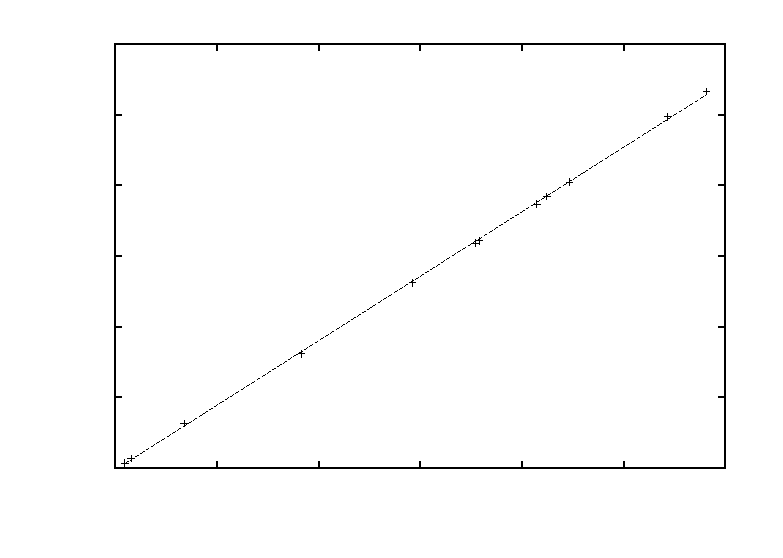
\includegraphics{g1}}%
    \gplfronttext
  \end{picture}%
\endgroup

\end{center}
\caption{Kalibrační křivka spektrometru}
\label{kal}
\end{figure}

Pro další úkol jsem ještě doměřil hodnoty pro žlutou část spektra v druhém řádu. Hodnoty jsou v tabulce \ref{T5}.
\begin{table}
$$
\begin{array}{|c|c|c|c|c|}
\hline
n&  \psi_+& -\psi_-& |\psi_+-\psi_-|/2& \lambda/\mbox{nm} \\ \hline
1&  44\st 45'&  43\st 19'&  44\st 2'& 574\pm 3\\ \hline
2&  45\st 2'&   43\st 32'&  44\st 17'& 577\pm 3\\ \hline
\end{array}
$$
\caption{Hodnoty žlutých spektrálních čar druhého řádu.}
\label{T5}
\end{table}

Dle vztahu \ref{D} a z definice jsem vypočetl úhlovou disperzi mřížky ve žluté části spektra. Experimentální hodnoty jsou
\begin{eqnarray}
R_1&=&1.68\pm0.05 \mu\mbox{m}^{-1} \\
R_2&=&0.655\pm0.002 \mu\mbox{m}^{-1}
\end{eqnarray}
Teoretické hodnoty jsou
\begin{eqnarray}
R_{t1}&=&1.69\pm0.05 \mu\mbox{m}^{-1} \\
R_{t2}&=&0.656\pm0.002 \mu\mbox{m}^{-1}
\end{eqnarray}

\section{Diskuze}
Njevětší chyba celého měření vznikla při odečítání ze stupnice spektrometru. I při použití lupy byla velmi drobná, a proto se z nilnia velmi špatně odečítalo. 
Horší osvětlení stupnice tento efekt ještě umocnilo. I přes tuto chybu se celková relativní chyba pohybuje kolem jednoho procenta. Tabulkové hodnoty taktéž 
odpovídají naměřeným hodnotám. 

\section{Závěr}
Seřídil jsem spektrometr. \\
Stanovil jsem mřížkovou konstantu
\begin{eqnarray}
a=1650\pm10 \mbox{nm}
\end{eqnarray}
Odhadl jsem rozlišovací schopnost spektrometru
\begin{eqnarray}
R_{m1}&\approx&8900 \\
R_{m2}&\approx&17900
\end{eqnarray}
Proměřil jsem spektrum rtuťové výbojky. Výsledky jsou v tabulce \ref{Hg}. \\
Vytvořil jsem kalibrační křivku dle zadání. Výsledek je obrázek \ref{kal}. \\
Určil jsem úhlovou disperzi ve žluté části spektra rtuťové výbojky a dopočetl teoretické hodnoty. Výsledky jsou
\begin{eqnarray}
R_1&=&1.68\pm0.05 \mu\mbox{m}^{-1} \\
R_2&=&0.655\pm0.002 \mu\mbox{m}^{-1}\\
R_{t1}&=&1.69\pm0.05 \mu\mbox{m}^{-1} \\
R_{t2}&=&0.656\pm0.002 \mu\mbox{m}^{-1}
\end{eqnarray}
\end{document}
